\lab{Introduction to Parallel Computing}{Intro to Parallel Computing}
\objective{A great deal of modern problems involve such a large number of computations that running them on a single processor becomes either impractical or impossible. However, most computers now have multiple  processor cores which can allow various processes to run simultaneously. For even more massive computations, computers can be grouped into clusters that combine both memory and processing power. In this lab, we explore the basic principles of parallel computing by analyzing the cluster setup, the standard parallel commands, and code designs that fully utilize available resources. All concepts are taught using the {\texttt{\em iPyParallel}} Python package.}

\begin{comment}
For most computer programs, one processor suffices to run the program effectively. Many computers, however, have more than one processor in order to allow for efficient multitasking. For more computationally expensive code, it may be beneficial to utilize more than one of the machine's processors so that the code can run faster. This lab teaches about \li{ipyparallel}, a python module that allows users to directly access and run code on multiple processors at the same time.
\end{comment}

\label{lab:parallel1}

\section*{Why Parallel Computing?}
Many modern challenges in data science and mathematics involve enormous computational tasks.
In order to overcome these obstacles, faster processors are constantly being developed to improve a computer's capacity.
However, making faster processors involves making their transistors, and consequently the processors, smaller. 
This is a problem because it is difficult to dissipate the heat of a small processor
Thus, there has been a consistent push in the past few decades to \emph{parallelize} computations using multiple processors for greater speed.
Though there are many different architectures for parallel computing, essentially, a \emph{supercomputer} or \emph{computer cluster} is a group of normal computers that share their processors and memory for greater performance.

In the majority of circumstances, these processors communicate with each other and coordinate their tasks with a message passing system. 
The details of the most common message passing interface, or MPI, will be the topic of the next lab.
However, there are basic commands used for parallel programming that are shared in both MPI and in the Python module \li{iPyParallel}. 
This lab focuses on exploring the basic principles of computing clusters as well as those shared basic commands.

\section*{Serial Execution vs. Parallel Execution}
%Up to this point, all the programs you have written are executed one line at a time, or in \emph{serial}.
\emph{Serial} programs are those that are executed one piece at a time.
This can be visualized as a program that runs all of its computations on a single processor or core.
Figure \ref{fig:htop} visualizes what this would look like by using the Linux command \li{htop}.
This command shows which programs are running, how many resources they are using up, and how much each processor core is running.

\begin{figure}[!tbp]
  \begin{subfigure}[b]{0.49\textwidth}
    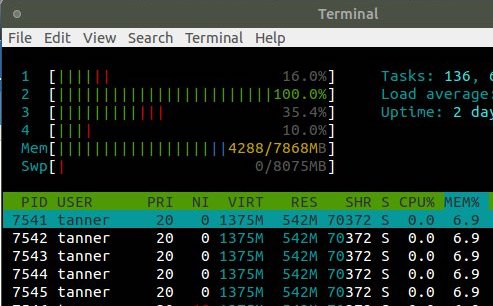
\includegraphics[width=\textwidth]{figures/activenew.jpg}
    \caption{Serial}
  \end{subfigure}
  \hfill
  \begin{subfigure}[b]{0.49\textwidth}
    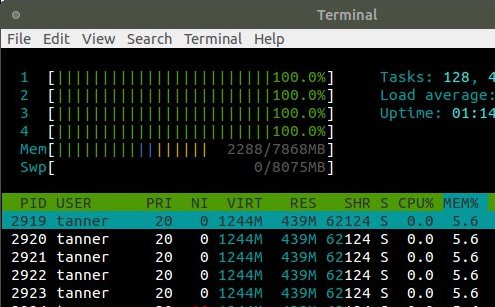
\includegraphics[width=\textwidth]{figures/cluster_activenew.jpg}
    \caption{Parallel}
  \end{subfigure}
  \caption{In the serial implementation, one core is running the program. In the parallel, it is split across all cores.}
  \label{fig:htop}
\end{figure}


%The following exercise will help visualize the serial process of a program.

%As was seen in the previous exercise, only one or two of the cores was carrying the load at a time, which means that only a fraction of the computer's resources are being used.
When running a program in serial, only a fraction of the computer's resources are being used.
This can be beneficial for smooth multitasking on a personal computer because programs can run uninterrupted on their own core.
However, to reduce the runtime of large computations, it is beneficial to devote all of a computer's resources (or the resources of many computers) to a program.
In theory, this parallelization can allow programs to run $N$ times faster where $N$ is the number of processors or processor cores that can be accessed.
Due to the necessity for communication, coordination, and travel time on wires, that improvement is not realistic, but the difference is substantial.

\section*{Basic Parallel Architecture}
There are several common architectures that combine computing resources for parallel processing.
Each architecture has a different protocol for sharing memory and processors between computing \emph{nodes}, which are the different simultaneous processing areas.
Each also offers unique advantages for the type of processing being completed.
However, the parallel commands used with each are very similar.

The following exercises will be based on the standard architecture in the \texttt{iPyParallel} module, which gives each node its own processing and memory space.
Once constructed, the nodes are coordinated with a master process.

\subsection*{The \texttt{iPyParallel} Architecture}
The \texttt{iPyParallel} architecture can be better understood as a \emph{controller} that distributes messages (or commands) and \emph{engines} that receive the messages and run the processes.
The controller is comprised of a hub to manage communications and schedulers to assign processes to the engines.
Engines are distributed across computers or processor cores and have the sole task of running their assigned commands.
A diagram of the pieces of this architecture can be seen in Figure \ref{fig:ipyarch}.

\begin{figure}[H]
    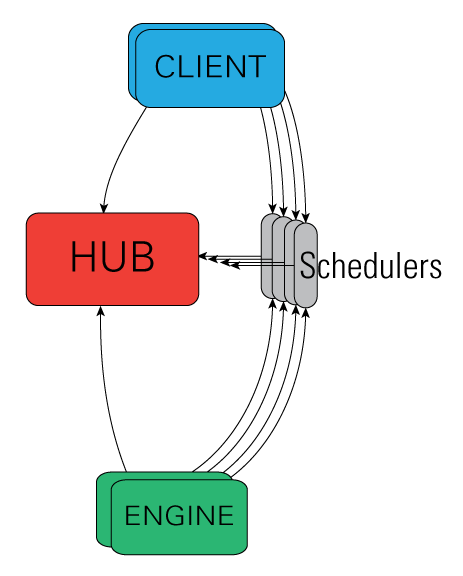
\includegraphics[width=.4\textwidth]{figures/ipyarch.png}
\caption{An outline of the pieces of the \texttt{iPyParallel} architecture. Retrieved from official documentation at \url{https://ipyparallel.readthedocs.io/en/latest/intro.html\#architecture-overview}.}
\label{fig:ipyarch}
\end{figure}

To initialize this architecture, \texttt{iPyParallel} must be installed on the machine.
Further instructions for installation can be found in the Additional Material section at the end of the lab.

\subsection*{Setting up a Cluster}
In order to allow for personal experimentation, the cluster setup for this lab will consist of a single machine with multiple processor cores.
%%%%%%%%%%%%%%%%%%%%%%%%%%%%%%%%%%%%%%%%%%%%%%%%%%%%%%%%%%%%%%%%%%%%%%%%%%%%%%%%%%%%%%%%%%%%%%%%%%%%%%%%%%%%%%%%%%%
However, further information on how to connect multiple machines is contained in Additional Material.

\subsubsection*{The Controller}
To initialize a controller on a machine, run the following command in a terminal window:
\begin{lstlisting}[style=ShellInput]
$ ipcontroller start
\end{lstlisting}

This command will start a controller process in the directory in which it was run and can be stopped by using \texttt{Ctrl+C}.
By default, this controller uses JSON files contained in \path{UserDirectory/.ipython/profile-default/security/} to determine it's settings.
Once a controller is running, it acts like a server listening for client connections from engine processes.

\subsubsection*{The Engines}
To start an engine process, run the following in a new terminal window:
\begin{lstlisting}[style=ShellInput]
$ ipengine start
\end{lstlisting}

This command starts an engine client program in the directory in which it was run and by default connects to a controller with the settings defined in the JSON files of \path{UserDirectory/.ipython/profile-default/security/}.
There is no limit to the number of engines that can be started in their own terminal windows and connected to the controller, however, it is recommended that only as many engines are started as there are cores to maximize efficiency. 
Once started, each engine has its own ID number on the controller that is used for communication.

\begin{warn}
Engines must be in the same directory as any additional Python files that will to be imported.
For example, if \li{program.py} imports \li{function} from \li{important.py}, then \li{important.py} has to be in the same directory as the engine.
This does not apply to installed Python modules.
\end{warn}

\subsubsection*{The Cluster}
Once a controller and its engines have been started and are connected, a cluster has successfully been established.
The controller will now be able to distribute messages to each of the engines, which will compute with their own processor and memory space and return their results to the controller.

Instead of starting the controller and engines in separate terminal windows as previously shown, there is a method to start the controller and engines in one terminal window by running:
\begin{lstlisting}[style=ShellInput]
$ ipcluster start # By default assigns an engine to each processor core.
$ ipcluster start --n 4 # Starts a cluster with 4 engines.
\end{lstlisting}

The terminal command \texttt{ctrl+c} can be used to stop the terminal window process and \li{ipcluster stop} can be used to entirely stop the cluster.
Though the previous instructions to start a controller and engines in separate terminal windows are less convenient, having unique terminal windows for the engines allows a user to see individual errors in detail and is more convenient for starting a cluster of multiple computers.

\begin{info}
Jupyter notebooks also have a \bf{Clusters} tab in which clusters can be initialized using an interactive GUI.
To enable this tab, run:
\begin{lstlisting}[style=ShellInput]
$ ipcluster nbextension enable
\end{lstlisting}
\end{info}


\section*{The $\texttt{iPyParallel}$ Interface}
Since Python is a relatively slow scripting language, and since the main purpose of parallel computing is to speed up run time, most parallel computing is done in a language other than Python.
However, it is still fairly easy to speed up run time and to test parallel code logic in the \texttt{iPyParallel} environment.
Once a cluster has been started with a controller and engines, \texttt{iPyParallel} has a specific interface that allows for communication. 
This interface allows a user to specify what happens on each core and how those cores communicate, which is the heart of all parallel computing.

A controller is manipulated through a \li{Client} object, which can be initialized as follows:

\begin{lstlisting}
>>> from ipyparallel import Client
>>> client = Client()
>>> client.ids # If you had four processors, the output would be as follows.
<< [0, 1, 2, 3] >>
\end{lstlisting}

Once the client object has been created, it can be used to create one of two classes: a \li{DirectView} or a \li{LoadBalancedView}.
These views allow for messages to be sent to collections of engines simultaneously.
A \li{DirectView} allows for total control of task distribution while a \li{LoadBalancedView} automatically tries to spread out the tasks to be equal on all engines.
The remainder of the lab will be focused on the \li{DirectView} class which can be initialized as follows:

\begin{lstlisting}
>>> dview = client[:] # Group all engines into a Direct View.
>>> dview2 = client[:2] # Group engines 0,1, and 2 into a Direct View.
\end{lstlisting}

There is also a \li{targets} object which can be set as a \li{DirectView} variable or as a parameter in functions.
It allows for a subgroup of the Direct View to be specified for subsequent actions.
It is accessed as follows.

\begin{lstlisting}
# Target only engines 0 and 2 until changed.
>>> dview.targets = [0,2]
# To revert to all engines,
>>> dview.targets = None
\end{lstlisting}

Since each engine has its own namespace, we must ensure that the desired modules are imported in each engine.
There is more than one way to do this. 

For example, the following commands import NumPy to all engines simultaneously.

\begin{lstlisting}
>>> with dview.sync_imports():
...	import numpy
>>> dview.execute('''np = numpy''')
# Or simply,
>>> dview.execute('''import numpy as np''')
\end{lstlisting}

\begin{problem}
Write a function \li{initialize()} that initializes a Client object, creates a Direct View with all available engines, and imports \li{scipy.sparse as spar} on all engines.
\end{problem}

\section*{Basic Parallel Commands in $\texttt{iPyParallel}$}
%The basic framework for \li{iPyParallel} revolves around a \li{DirectView} or a \li{LoadBalancedView}.
%A \li{DirectView} is the object through which we can communicate with each of the engines individually and gives us control over which variables are pushed to each engine and what functions are performed. 
%A \li{LoadBalancedView} takes the commands that are being executed and does its best to distribute the load evenly across all engines.

%For the purposes of learning how each engine works, we will focus on the \li{DirectView} in this lab. 
%To initialize a \li{DirectView}, run the following code:
The \li{DirectView} gives control of the available engines to the user and allows them to interact with each engine individually or as a group.
Each engine can be likened to its own iPython terminal with a namespace in which variables, functions, and imports must be defined individually.

\subsection*{Blocking vs. Non-Blocking}
Parallel commands can be implemented in a \emph{blocking} or \emph{non-blocking} format.
They are defined as follows:
\begin{list}{}{}
\item \textbf{Blocking} - The command is sent and the program halts until the answer is received. 
This format is usually ideal for problems in which each node is performing the same task.
\item \textbf{Non-Blocking} - The command is sent and an object is immediately returned with a flag that shows whether the response is ready or not.
This allows for greater synchronization between nodes and for large blocks of code to be executed without needing to wait for responses.
\end{list}

Though difficult to grasp initially, this is an extremely important part of parallel processing.
An example of the benefits of blocking and non-blocking is demonstrated below.

\begin{lstlisting}
# The following is a blocking implementation of a for loop
>>> dview.execute('''import numpy as np''')
>>> results = []
>>> for i in range(1000):
...	results.append(dview.apply_sync(lambda x: np.<<sum>>(np.random.random(x)),i))
''' 
The for loop waits until each answer is gathered, then appends them. This 
blocking method takes 16.8495s with 4 engines.
'''

# The following is a non-blocking implementation
>>> results2 = []
>>> for j in range(1000):
...	results2.append(dview.apply_async(lambda x: np.sum(np.random.random(x)),j))
>>> results2 = [x.get() for x in results2]
''' 
In this example, the for loop appends an ASyncResult object to the list
and continues the loop. The answers are later retrieved after they have
finished processing. Though this method has two for loops, it takes only
12.9706s with 4 engines.
'''
\end{lstlisting}

As was demonstrated above, when non-blocking is used, commands can be continuously sent to engines before they have finished their previous task.
This allows them to begin their next task without waiting to send their calculated answer and receive a new command.
However, this requires a design that incorporates check points to retrieve answers and enough memory to store response objects.

There is a \li{DirectView} variable called \li{block} that controls the default format.
Blocking can also be entered as a parameter in most functions.
The variable is accessed as follows.

\begin{lstlisting}
# Make blocking default
>>> dview.block = True
\end{lstlisting}

\subsection*{Variables on Different Engines}
%When using multiple processors, you can imagine each engine running its own iPython terminal with its own namespace.
All variables must be initialized on each individual engine.
There are a few methods to do this.

\subsubsection*{Push and Pull}
When variables are sent to engines or retrieved from them, the methods \li{push} and \li{pull} are used.
The following demonstrates these methods.

\begin{lstlisting}
# To share the variables 'a' and 'b' across all engines
>>> dview['a'] = 10
>>> dview['b'] = 5
# These two commands are shorthand for
>>> dview.push({'a':10, 'b':5}, block=True)

# To ensure the variables are on engine 0
>>> client[0]['a']
<< 10 >>

# On all engines
>>> dview['a']
<< [10, 10, 10, 10] >>
# Which is shorthand for
>>> dview.pull('a', block=True)
\end{lstlisting}

The above examples demonstrate simple blocking methods of sending variables to the engines.
There are also non-blocking methods that return an \li{ASyncResult} object that has commands to access its content.
This is demonstrated as follows:

\begin{lstlisting}
>>> res = dview.pull(['a', 'b'],block=False)
>>> res.ready()
<< True >>
>>> res.get()
<< [[10, 5], [10, 5], [10, 5], [10, 5]] >>
\end{lstlisting}

A table of ASyncResult methods are included in Table \ref{table:asyncresult}.

\begin{table}[H] % ASyncResult methods
\centering
\begin{tabular}{l|l}
Class Method & Description
\\ \hline
\li{wait(timeout)} & Wait until the result is available or until \li{timeout} seconds pass.\\& This method always returns \texttt{None}. \\
\li{ready()} & Return whether the call has completed. \\
\li{successful()} & Return whether the call completed without raising an exception.\\& Will raise \texttt{AssertionError} if the result is not ready. \\
\li{get(timeout)} & Return the result when it arrives. If \li{timeout} is not \texttt{None} and the \\& result does not arrive within \li{timeout} seconds then \li{TimeoutError}\\& is raised.
\end{tabular}
\caption{All information from \url{https://ipyparallel.readthedocs.io/en/latest/details.html\#AsyncResult}.}
\label{table:asyncresult}
\end{table}

\begin{problem}
Write a function \li{variables(dx)} that accepts a dictionary of variables. 
Create a \li{Client} object and a \li{Direct View} and distribute the variables.
Then, pull the variables in both a blocking and non-blocking format.
Return the resultant objects of both formats.
\end{problem}

\subsubsection*{Scatter and Gather}
There are also ways to take an array of elements and split them up between all of the Direct View engines.
This is called \emph{scattering}.
A simple example is contained below.

\begin{lstlisting}
>>> import numpy as np
>>> one = [1, 2, 3, 4]
>>> two = np.array([1, 2, 3, 4])
>>> dview.scatter("one_part", one, block=True)
>>> dview["one_part"]
<< [[1], [2], [3], [4]] >>
>>> dview.scatter("two_part", one, block=True, targets=[0,2])
>>> dview["two_part"]
<< [array([1, 2]), array([3, 4])] >>
\end{lstlisting}

Collecting scattered pieces into one object is called \emph{gathering}.
An example is contained below.

\begin{lstlisting}
>>> print(dview.gather("one_part", block=True))
<< [1, 2, 3, 4] >>
>>> print(dview.gather("two_part", block=True,targets=[0,2]))
<< array([1, 2, 3, 4]) >>
\end{lstlisting}

This method of distributing and collecting a dataset is the foundation of the MapReduce algorithm that is prominent in modern Data Science.

\subsection*{Methods for Execution}
To execute functions on each of the engines, we can use a few different functions.
Though not syntactically the same as commercial parallel programs, the \li{iPyParallel} functions perform similarly and are as follows.

\subsubsection*{Execute}
The execute method is the simplest method for executing commands on parallel engines.
It accepts a string with exact syntax for a method to be complete.
Examples are as follows.
The \li{htop} command should be used to compare against serial methods.

\begin{lstlisting}
>>> dview.execute('''
... import numpy as np
... rand = np.random.random
... c = np.sum(rand(a+b))
... ''')
>>> dview['c']
<< [7.9619371, 7.3431609, 7.4818468, 8.2783728] >>

# More involved example
>>> dview.scatter("p1", list(range(4)), block=True)
>>> dview.scatter("p2", list(range(10,14)), block=True)
>>> dview["p1"]
<< [[0], [1], [2], [3]] >>
>>> dview["p2"]
<< [[10], [11], [12], [13]] >>
>>> dview.execute('''
... def adding(a,b):
...     return a+b
... result = adding(p1[0],p2[0])
... ''')
<< <AsyncResult: execute:finished> >>
>>> dview['result']
<< [10, 12, 14, 16] >>
\end{lstlisting}

Though primitive, this method functions well for simple procedures.
More intricate methods follow.

\subsubsection*{Apply}
The \texttt{apply} method is the simplest function distributor for the \texttt{iPyParallel} interface.
It accepts a function and the arguments that correspond with the function and distributes it to the engines.
It has two children, \li{apply_sync} which blocks and \li{apply_async} which doesn't block.
There is no blocking parameter for these functions.
An example follows.

\begin{lstlisting}
# apply_sync always blocks
>>> dview.apply_sync(lambda x: a+b+x, 20)
<< [35, 35, 35, 35] >>

# apply_async never blocks
>>> def double_add(x,y):
...     return 2*x + 2*y
>>> answer = dview.apply_async(double_add,5,7)
>>> answer.ready()
<< True >>
>>> answer.get()
<< [24, 24, 24, 24] >>
\end{lstlisting}

Note that the engines can access their local variables in any of the execution methods.

\begin{problem}
Using one of the \texttt{apply} methods, write a function \li{apply_dist(n=1000000)} that prints the mean, max, and min of $n$ draws on each engine from the standard normal distribution.
For example if you have four engines running, your output should look like:
\begin{lstlisting}
<< means = [0.0031776784, -0.0058112042, 0.0012574772, -0.0059655951] >>
<< maxs = [4.0388107, 4.3664958, 4.2060184, 4.3391623] >>
<< mins = [-4.1508589, -4.3848019, -4.1313324, -4.2826519] >>
\end{lstlisting}
\end{problem}


\begin{problem}
Using the function you wrote in the previous problem, compare the time it takes to run the function with parallel computing to the time it takes to run the function serially.
That is, time how long it takes to run the function on all of your machine's engines simultaneously and how long it takes to run the function in a \texttt{for} loop $n$ times, where $n$ is the number of engines on your machine.
Print the results for 1,000,000; 5,000,000; 10,000,000; and 15,000,000 samples.
You should notice an increase in efficiency as the problem size increases.
\end{problem}

\subsubsection*{Map}
The \li{iPyParallel} module also has a generalized version of the Python function \texttt{map} that combines \texttt{apply} with \li{scatter} and \li{gather}.
Simply put, it accepts a dataset, splits it between the engines, executes a function on the given elements, returns the results, and combines them into one object.
The \texttt{map} function does have a blocking parameter, but, like the \texttt{apply} function, it also has children, \li{map_sync} and \li{map_async}.
A couple of examples follow.

\begin{lstlisting}
# Single input function
>>> num_list = [1,2,3,4,5,6,7,8]
>>> def triple(x):
...     return 3*x
>>> answer = dview.<<map>>(triple, num_list, block=True)
<< [3, 6, 9, 12, 15, 18, 21, 24] >>

# Multiple input function
>>> def add_three(x,y,z):
...     return x+y+z
>>> x_list = [1,2,3,4]
>>> y_list = [2,3,4,5]
>>> z_list = [3,4,5,6]
>>> dview.map_sync(add_three, x_list, y_list, z_list)
<< [6, 9, 12, 15] >>

# Engine variable function
>>> def mult(x):
...		return a*x
>>> answer = dview.map_async(mult, x_list)
>>> answer.get()
<< [10, 20, 30, 40] >>
\end{lstlisting}

The \texttt{map} function also represents a key component in the MapReduce algorithm and is very important.

There are additional magic methods supplied by \li{iPyParallel} that make some of these operations easier.
These methods are contained in the Additional Material section.
More information on \li{iPyParallel} architecture, interface, and methods at \url{https://ipyparallel.readthedocs.io/en/latest/index.html}.


\section*{Parallel Computing}
To this point, the examples of what parallel computing can do may not seem too interesting since each engine is basically producing the same result.
There are, however, circumstances in which the engines return different results.
In these situations, parallel computing can drastically speed up processing.

\begin{problem}
In a previous lab, latitude and longitude points of recycle bins and addresses in New York City were analyzed to find the address furthest from a recycle bin.
To do so, a KDTree was implemented with the following:

\begin{lstlisting}
>>> from scipy.spatial import KDTree
# Columns should be latitude then longitude
>>> lat_long_array = np.array([ [1,2], [2,3], [3,4] ])
>>> tree = KDTree(lat_long_array)
>>> sample_point = np.array([2,5])
# Queries can be made with
>>> q = tree.query(sample_point)
>>> q
<< (1.4142135623730951, 2) >>
\end{lstlisting}

Write a function called \li{bin_parallel} that uses a parallel implementation to find the furthest address from a recycle bin.
Return the furthest address, its closest bin, and the runtime of your function as a tuple.

The necessary data points have been given as \li{recycle_bins.npy} and \li{ny_addr.npy} with latitude and longitude as rows and records as columns.
\end{problem}

In theory, using parallel computing for these simple problems should be approximately $N$ times faster, where $N$ is the number of engines you are using.
In practice, however, the scaling is not quite linear.
This is due in part to the controller running on one of the engines, the computer's standard processes still running, and the overhead of controller and engine communication.

\subsection*{Applications}
Parallel computing, when used correctly, is one of the best ways to speed up the run time of an algorithm.
As a result, it is very commonly used today and has many applications, such as the following:
\begin{itemize}
\item Graphic rendering
\item Facial recognition with large databases
\item Numerical integration
\item Calculating Discrete Fourier Transforms
\item Simulation of various natural processes (weather, genetics, etc.)
\item Natural language processing
\end{itemize}
In fact, there are many problems that are only possible to solve through parallel computing because solving them serially would take too long. 
In these types of problems, even the parallel solution could take years. 
Some brute-force algorithms, like those used to crack simple encryptions, are examples of this type of problem.

The problems mentioned above are well suited to parallel computing because they can be manipulated in such a way that running them on multiple processors results in a significant run time improvement.
Manipulating an algorithm to be run with parallel computing is called \emph{parallelizing} the algorithm. 
When a problem only requires very minor manipulations to parallelize, it is often called \emph{embarrassingly parallel}.
Typically, an algorithm is embarrassingly parallel when there is little to no dependency between results.
Algorithms that do not meet this criteria can still be parallelized, but there is not always a significant enough improvement in run time to make it worthwhile. 
For example, calculating the Fibonacci sequence using the usual formula, F($n$) = F($n-1$) + F($n-2$), is poorly suited to parallel computing because each element of the sequence is dependent on the previous two elements.


\begin{problem}
Consider the problem of numerical integration using the trapezoidal rule, depicted in Figure \ref{fig:traprule}.
Recall the following formula for estimating an integral using the trapezoidal rule,
\[
\int_{a}^b f(x) dx \approx \frac{h}{2} \sum_{k=1}^N (f(x_{k+1}) + f(x_k)),
\]
where $x_k$ is the $k$th point, and $h$ is the distance between any two points (note they are evenly spaced).

Note that estimation of the area of each interval is independent of all other intervals. 
As a result, this problem is considered to be embarrassingly parallel.

Write a function called \li{parallel_trapezoidal_rule()} that accepts a function handle to integrate, bounds of integration, and the number of points to use for the approximation. 
Utilize what you have learned about parallel computing to parallelize the trapezoidal rule in order to estimate the integral of $f$. 
That is, evenly divide the points among all available processors and run the trapezoidal rule on each portion simultaneously.
The sum of the results of all the processors will be the estimation of the integral over the entire interval of integration.
Return this sum. 

\begin{figure}[H]

\begin{center}
		
\begin{tikzpicture}[scale=1.5]
%Draw the axes
\draw[->,>=stealth',thick] (-.5,0) -- (5,0);
\draw[->,>=stealth',thick] (0,-.5) -- (0,5);
%Draw the ticks and labels
\foreach \x/\t in {.5/x_1,1.5/x_2,2.5/x_3,3.5/x_4,4.5/x_5} \draw (\x,-3pt) -- (\x,0) node[anchor=north, yshift=-.25cm] {$\t$}; 
%Labels
%\node[align=center] at (1.3,4) {Trapezoid Rule\\Uniform Partitioning};
\node[anchor=east,xshift=-.2cm] at (0,4.5) {$y$};
\node[anchor=north,yshift=-.25cm] at (5,-.2) {$x$};
\node[yshift=-.25cm] at (3,3.5) {$y=f(x)$};
%Draw the curve
\draw[thick] (.5,2) sin (1.5,2.7) cos (2.5,2.5) sin (3.5,2.3) cos (4.5,3);
%Draw the faded vertical lines
\foreach \x/\y in {.5/2,1.5/2.7,2.5/2.5,3.5/2.3,4.5/3} \draw[help lines] (\x,0) -- (\x,\y);
%The h measure and label
\draw[thick] (1.5,1.4) -- (1.5,1.6) |- (2,1.5) node[below] {$h$} -| (2.5,1.4) -- (2.5,1.6) ;
%Draw the red lines
\foreach \x/\y/\s/\t in {.5/2/1.5/2.7,1.5/2.7/2.5/2.5,2.5/2.5/3.5/2.3,3.5/2.3/4.5/3} \draw[red,thick] (\x,\y) -- (\s,\t);

\end{tikzpicture}
\end{center}
\label{fig:traprule}
\caption{A depiction of the trapezoidal rule with uniform partitioning.}
\end{figure}


\end{problem}


\subsection*{Intercommunication}
The phrase \emph{parallel computing} refers to designing an architecture and code that makes the best use of computing resources for a problem.
Occasionally, this will require nodes to be interdependent on each other for previous results.
This contributes to a slower result because it requires a great deal of communication latency, but is sometimes the only method to parallelize a function.
Although important, the ability to effectively communicate between engines has not been added to \texttt{iPyParallel}.
It is, however, possible in an MPI framework and will be covered in a later lab.

% Old problem
%\begin{problem}
%All of the examples that we have done in this lab up to this point may have seemed quite simplistic. However, we will now apply all these examples to a real-world example.
%
%Many natural language processing (NLP) problems naturally extend to a parallel computing architecture. In many situations, we will have a function we want to apply to a piece of text, whether that be a sentence, paragraph, or an entire document. An efficient way to handle these problems is to scatter the data to all available engines, perform the calculations, then gather the results.
%
%The introductory step to latent symantic analysis is to create a occurance matrix based on the bag-of-words model. At a high level, the bag-of-words model gives us insight as to the topic of a given document. It can also be used to measure the similarity between two documents.
%
%The occurrence matrix has the ids for the different documents as the rows and the different words in the vocabulary as the columns. Then the $ij$-th entries of this matrix is the number of times the $j$-th word appears in the $i$-th document. For example, consider the following example:
%
%Say we have the following 4 pieces of text:
%\begin{enumerate}
%    \item the rose is red
%    \item the violet is blue
%    \item my car is red
%    \item i have a red rose and a red car
%\end{enumerate}
%
%It is common to remove \emph{stopwords} or the most common words in the language. We can get a list of stopwords by running:
%\begin{lstlisting}
%>>> from nltk.corpus import stopwords
%>>> set_stopwords = set(stopwords.words('english'))
%\end{lstlisting}
%
%After removing the stopwords, the resulting occurrence matrix would be:
%\begin{lstlisting}
%      'blue' 'car' 'red' 'rose' 'violet'
%doc1     0     0     1      1       0
%doc2     1     0     0      0       1
%doc3     0     1     1      0       0
%doc4     0     1     2      1       0
%\end{lstlisting}
%
%Notice that the columns contain all the non-stopwords that were used throughout all the documents combined.
%
%The \li{state_union.zip} file contains all of the State of the Union addresses from 1945-2006. For this problem, leverage the power of parallel computing to create an occurrence matrix where the rows are the different State of the Union addresses and the columns are the words in the collective vocabulary. There are many ways to tackle this problem, so we will leave it open-ended. However, we strongly recommend that you base your solution around the \li{scatter()} and \li{gather()} methods.
%
%For the sake of grading, order the rows chronologically and the columns in alphabetical order. Also, as you can imagine, this matrix will end up being fairly sparse, so it is more efficient to use \li{scipy.sparse} matrices.
%\end{problem}

\newpage
\section*{Additional Material}

\subsection*{Installation and Initialization of $\texttt{ipyparallel}$}

If you have not already installed \li{ipyparallel}, you may do so using the conda package manager.

\begin{lstlisting}[style=ShellInput]
$ conda update conda
$ conda update anaconda
$ conda install ipyparallel
\end{lstlisting}

\subsection*{Clusters of Multiple Machines}
Though setting up a computing cluster with \texttt{iPyParallel} on multiple machines is similar to a cluster on a single computer, there are a couple of extra considerations to make.
The majority of these considerations have to do with the network setup of your machines, which is unique to each situation.
However, some basic steps have been taken from \url{https://ipyparallel.readthedocs.io/en/latest/process.html} and are outlined below.

\subsubsection*{SSH Connection}
When using engines and controllers that are on separate machines, their communication will most likely be using an SSH tunnel.
This \emph{Secure Shell} allows messages to be passed over the network.

In order to enable this, an SSH user and IP address must be established when starting the controller.
An example of this follows.

\begin{lstlisting}[style=ShellInput]
$ ipcontroller --ip=<controller IP> --user=<user of controller> --enginessh=<user of controller>@<controller IP>
\end{lstlisting}

Engines started on remote machines then follow a similar format.

\begin{lstlisting}[style=ShellInput]
$ ipengine --location=<controller IP> --ssh=<user of controller>@<controller IP>
\end{lstlisting}

Another way of affecting this is to alter the configuration file in \path{UserDirectory/.ipython/profile-default/security/ipcontroller-engine.json}.
This can be modified to contain the controller IP address and SSH information.

All of this is dependent on the network feasibility of SSH connections.
If there are a great deal of remote engines, this method will also require the SSH password to be entered many times.
In order to avoid this, the use of SSH Keys from computer to computer is recommended.


\subsection*{Magic Methods \& Decorators}
To be more usable, the \texttt{iPyParallel} module has incorporated a few magic methods and decorators for use in an interactive iPython or Python terminal.

\subsubsection*{Magic Methods}
The \texttt{iPyParallel} module has a few magic methods that are very useful for quick commands in iPython or in a Jupyter Notebook.
The most important are as follows.
Additional methods are found at \url{https://ipyparallel.readthedocs.io/en/latest/magics.html}.

\begin{list}{}{}
\item \textbf{\%px} - This magic method runs the corresponding Python command on the engines specified in \li{dview.targets}.
\item \textbf{\%autopx} - This magic method enables a boolean that runs any code run on every engine until \li{\%autopx} is run again.
\end{list}

Examples of these magic methods with a client and four engines are as follows.

\begin{lstlisting}
# %px
In [4]: with dview.sync_imports():
   ...:     import numpy
   ...:     
importing numpy on engine(s)
In [5]: \%px a = numpy.random.random(2)

In [6]: dview['a']
Out[6]: 
[array([ 0.30390162,  0.14667075]),
 array([ 0.95797678,  0.59487915]),
 array([ 0.20123566,  0.57919846]),
 array([ 0.87991814,  0.31579495])]
 
 # %autopx
In [7]: %autopx
%autopx enabled
In [8]: max_draw = numpy.max(a)

In [9]: print('Max_Draw: {}'.format(max_draw))
[stdout:0] Max_Draw: 0.30390161663280246
[stdout:1] Max_Draw: 0.957976784975849
[stdout:2] Max_Draw: 0.5791984571339429
[stdout:3] Max_Draw: 0.8799181411958089

In [10]: %autopx
%autopx disabled
\end{lstlisting}
\subsubsection*{Decorators}
The \texttt{iPyParallel} module also has a few decorators that are very useful for quick commands.
The two most important are as follows:

\begin{list}{}{}
\item \textbf{@remote} - This decorator creates methods on the remote engines.
\item \textbf{@parallel} - This decorator creates methods on remote engines that break up element wise operations and recombine results.
\end{list}

Examples of these decorators are as follows.

\begin{lstlisting}
# Remote decorator
>>> @dview.remote(block=True)
>>> def plusone():
...	return a+1
>>> dview['a'] = 5
>>> plusone()
<< [6, 6, 6, 6,] >>

# Parallel decorator
>>> import numpy as np

>>> @dview.parallel(block=True)
>>> def combine(A,B):
...	return A+B
>>> ex1 = np.random.random((3,3))
>>> ex2 = np.random.random((3,3))
>>> print(ex1+ex2)
<< [[ 0.87361929  1.41110357  0.77616724]
 [ 1.32206426  1.48864976  1.07324298]
 [ 0.6510846   0.45323311  0.71139272]] >>
>>> print(combine(ex1,ex2))
<< [[ 0.87361929  1.41110357  0.77616724]
 [ 1.32206426  1.48864976  1.07324298]
 [ 0.6510846   0.45323311  0.71139272]] >>
 \end{lstlisting}
%\begin{info}
%If you are using a Jupyter Notebook, there is a built in magic function that is analagous to \li{dview.execute()}.
%If you put the \li{\%\%px} magic at the beginning of a cell of code, that cell of code will be executed on each engine. 
%This tool is very useful for designing and debugging parallel algorithms.
%\end{info}

\subsection*{Connecting \texttt{iPyParallel} with MPI}
The \texttt{iPyParallel} cluster can be imbued with the ability to interpret MPI commands.
More information on making this connection can be found at \url{https://ipyparallel.readthedocs.io/en/latest/mpi.html}.


%%%%%%%%%%%%%%%%%%%%%%%%%%% Old Problems %%%%%%%%%%%%%%%%%%%%%%%%%%%%%
\begin{comment}

%% 1
\begin{problem}
If you are working on a Linux or Mac computer, open a terminal and execute the \li{htop} command. (If \li{htop} is not on your system, install it using your default package manager). 
When opening this program, your terminal should see an interface similar to Figure \ref{fig:htop}. 
The numbered bars at the top represent each of the cores of your processor and the workload on each of these cores.

Now, run the following Python code with your terminal running \li{htop} still visible. 
The sole purpose of the following code is to create a computationally intensive function that runs for about 15 seconds.

\begin{lstlisting}
import numpy as np
for i in range(10000):
    np.random.random(100000)
\end{lstlisting}

You should have seen one or two (if your operating system has some built in load balancing) of the cores run substantially higher than the others. 
%It is also possible that you saw the load-carrying core switch midway through the execution of the file. 
This is an indicator that our script is being executed in serial -- one line at a time, one core at a time.
\end{problem}

\begin{figure}[H]
    \includegraphics[width=\textwidth]{figures/active.jpg}
\caption{An example of \li{htop} with a computationally intense python script running.}
\label{fig:htop}
\end{figure}


%% 2
\begin{problem}
Initialize an IPython cluster with an engine for each of your machines processor cores. 
As you did in the previous problem, open \li{htop}. 
Run the following code and examine what happens in htop.

\begin{lstlisting}
from ipyparallel import Client
client = Client()
dview = client[:]

dview.execute("""
import numpy as np
for i in range(10000):
    np.random.random(100000)
""")
\end{lstlisting}

The output of \li{htop} should appear similar to Figure \ref{fig:htop_cluster}. 
Notice that all of the processors are being utilized to run the script.
\end{problem}

\begin{figure}
    \includegraphics[width=\textwidth]{figures/cluster_active.jpg}
\caption{An example of \li{htop} with a computationally intense python script running in parallel.}
\label{fig:htop_cluster}
\end{figure}


%% 3
\begin{problem}
Now let's do a problem that is a bit more computationally intensive. 
Define the random variable $X$ to be the maximum out of $N$ draws from the standard normal distribution.
For example, one draw from $X$ when $N$ = 10 would be the maximum out of 10 draws from the normal distribution.
Write a function that accepts an integer $N$, takes 500,000 draws from this distribution ($X$), and plots the draws in a histogram.
The resulting histogram will approximate the p.d.f. of $X$.

Write your function in such a way that each engine will carry an equal load. Also write your function in such a way that it is flexible to the number of engines that are running. HINT: Remember that you can get a list of all available engines using \li{clients.ids}.
\end{problem}

\end{comment}